\section{Infrastructure as Code (IaC)}

\subsection{Importancia de IaC}

Infrastructure as Code consiste en describir la infraestructura (redes, bases de datos, contenedores, permisos) en archivos de código versionados, en lugar de crearla a mano desde la consola del proveedor. Sus ventajas para MisiOps son:

\begin{itemize}
    \item \textbf{Reproducibilidad}: \texttt{dev} y \texttt{prod} salen del mismo código y solo difieren en los parámetros declarados en \texttt{infra/lib/config.ts}. No hay configuración ``invisible'' hecha en la consola.
    \item \textbf{Revisión y trazabilidad}: cada cambio de infraestructura pasa por un PR, por el flujo SDD y por un pipeline de pruebas, igual que el código de la aplicación.
    \item \textbf{Pruebas antes de desplegar}: las propiedades de seguridad (base de datos privada, cifrado, secretos sin texto plano, rol de mínimo privilegio) se verifican con tests automáticos sobre la plantilla generada.
    \item \textbf{Despliegue y rollback automáticos}: CloudFormation aplica los cambios de forma transaccional y revierte si algo falla. Una nueva versión se despliega haciendo merge, sin pasos manuales.
\end{itemize}

La infraestructura se escribió con \textbf{AWS CDK en TypeScript} (\texttt{aws-cdk-lib} 2.273.0). CDK genera (\textit{synth}) plantillas de \textbf{AWS CloudFormation}, y CloudFormation es el servicio que crea, actualiza y revierte los recursos. Esta parte se desarrolló con el flujo SDD en \texttt{specs/012-aws-deployment/} y se integró con el PR \#178.

\subsection{Arquitectura de IaC y componentes}

\begin{figure}[H]
    \centering
    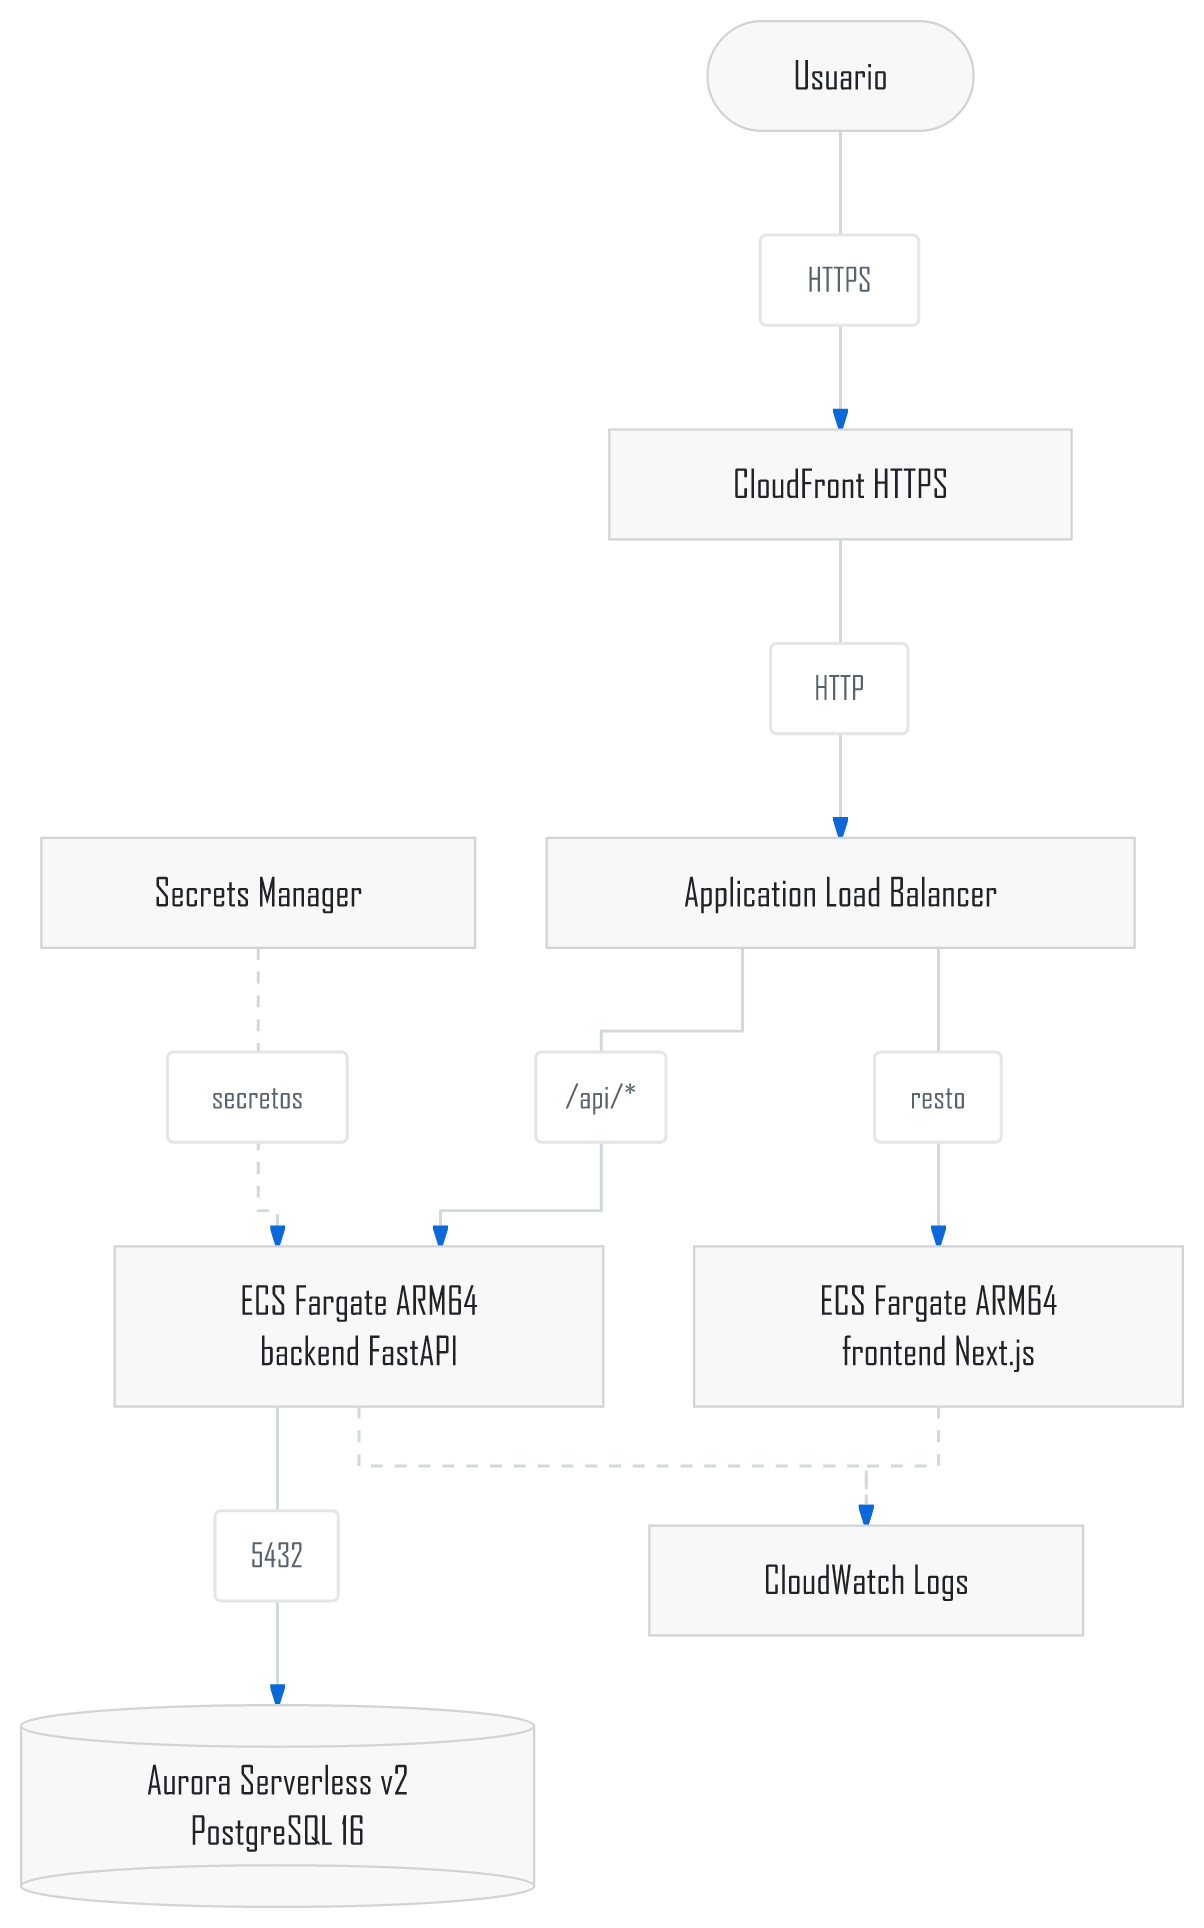
\includegraphics[width=0.5\textwidth]{figures/iac/iac-arch.png}
    \caption{Arquitectura en ejecución de MisiOps en AWS (región \texttt{us-east-1}), definida con CDK}
    \label{fig:iac-arch}
\end{figure}

El camino de despliegue (OIDC, ECR y CloudFormation) se muestra en la Figura~\ref{fig:iac-pipeline}. El código está en \texttt{infra/} y define dos tipos de stack:

\begin{table}[H]
    \centering
    \small
    \caption{Stacks de CloudFormation}
    \begin{tabularx}{\textwidth}{@{}p{3.3cm} p{3.2cm} X@{}}
        \toprule
        \textbf{Stack} & \textbf{Quién lo despliega} & \textbf{Contenido} \\
        \midrule
        \texttt{MisiOps-Foundation} & Un administrador, una vez & Proveedor OIDC de GitHub, rol de despliegue \texttt{MisiOpsGithubDeploy} y repositorios ECR \\
        \texttt{MisiOps-dev}, \texttt{MisiOps-prod} & El workflow \texttt{deploy} & VPC, Aurora Serverless v2, secretos, clúster y servicios ECS, ALB, CloudFront, logs y presupuesto \\
        \bottomrule
    \end{tabularx}
\end{table}

\begin{itemize}
    \item \textbf{CloudFront}: punto de entrada HTTPS con un dominio \texttt{*.cloudfront.net} generado; redirige HTTP a HTTPS y solo guarda en caché los recursos estáticos con hash (\texttt{/\_next/static/*}).
    \item \textbf{Application Load Balancer}: enruta por ruta. \texttt{/api/*}, \texttt{/openapi.json}, \texttt{/docs} y \texttt{/redoc} van al backend; el resto, al frontend.
    \item \textbf{ECS Fargate (ARM64/Graviton)}: un servicio para el backend FastAPI (puerto 8000) y otro para el frontend Next.js (puerto 3000), con 0.25 vCPU y 512 MiB cada uno. Cada servicio tiene \textit{deployment circuit breaker} con rollback automático.
    \item \textbf{Aurora Serverless v2 (PostgreSQL 16)}: en subredes aisladas, sin acceso público, cifrada, con escalado de 0 a 1 ACU y pausa automática tras 10 minutos sin uso. En \texttt{prod} tiene protección contra borrado y snapshot final.
    \item \textbf{Secrets Manager}: credenciales de la base de datos (generadas por el clúster) y \texttt{SECRET\_KEY}, inyectadas como secretos de ECS. Ningún secreto aparece en la plantilla ni en el repositorio.
    \item \textbf{ECR}: repositorios \texttt{misiops-backend} y \texttt{misiops-frontend} con tags inmutables (el SHA del commit) y escaneo al subir.
    \item \textbf{OIDC y rol de despliegue}: GitHub Actions obtiene credenciales temporales de una hora; no hay llaves de AWS guardadas en GitHub. El rol solo puede asumir los roles de CDK, subir imágenes a los dos repositorios y consultar stacks.
    \item \textbf{CloudWatch Logs} (30 días por servicio) y un \textbf{AWS Budget} de 60 USD al mes por entorno con alertas por correo.
    \item \textbf{VPC sin NAT}: las tareas usan subredes públicas con IP pública para descargar imágenes. Con esta decisión el costo en reposo queda en unos 48 USD al mes por entorno.
\end{itemize}

El siguiente extracto de \texttt{infra/lib/foundation-stack.ts} muestra cómo se restringe el rol de despliegue a este repositorio y a sus ramas o entornos:

\begin{lstlisting}[language=Java,caption={Confianza OIDC del rol de despliegue (extracto)}]
const subjects = [
  `repo:${githubRepo}:ref:refs/heads/develop`,
  `repo:${githubRepo}:ref:refs/heads/main`,
  `repo:${githubRepo}:environment:dev`,
  `repo:${githubRepo}:environment:prod`,
];
this.deployRole = new iam.Role(this, 'DeployRole', {
  roleName: 'MisiOpsGithubDeploy',
  maxSessionDuration: Duration.hours(1),
  assumedBy: new iam.OpenIdConnectPrincipal(provider, {
    StringEquals: { 'token.actions.githubusercontent.com:aud': GITHUB_OIDC_AUDIENCE },
    StringLike: { 'token.actions.githubusercontent.com:sub': subjects },
  }),
});
\end{lstlisting}

\subsection{Pipeline de CI/CD}

\begin{figure}[H]
    \centering
    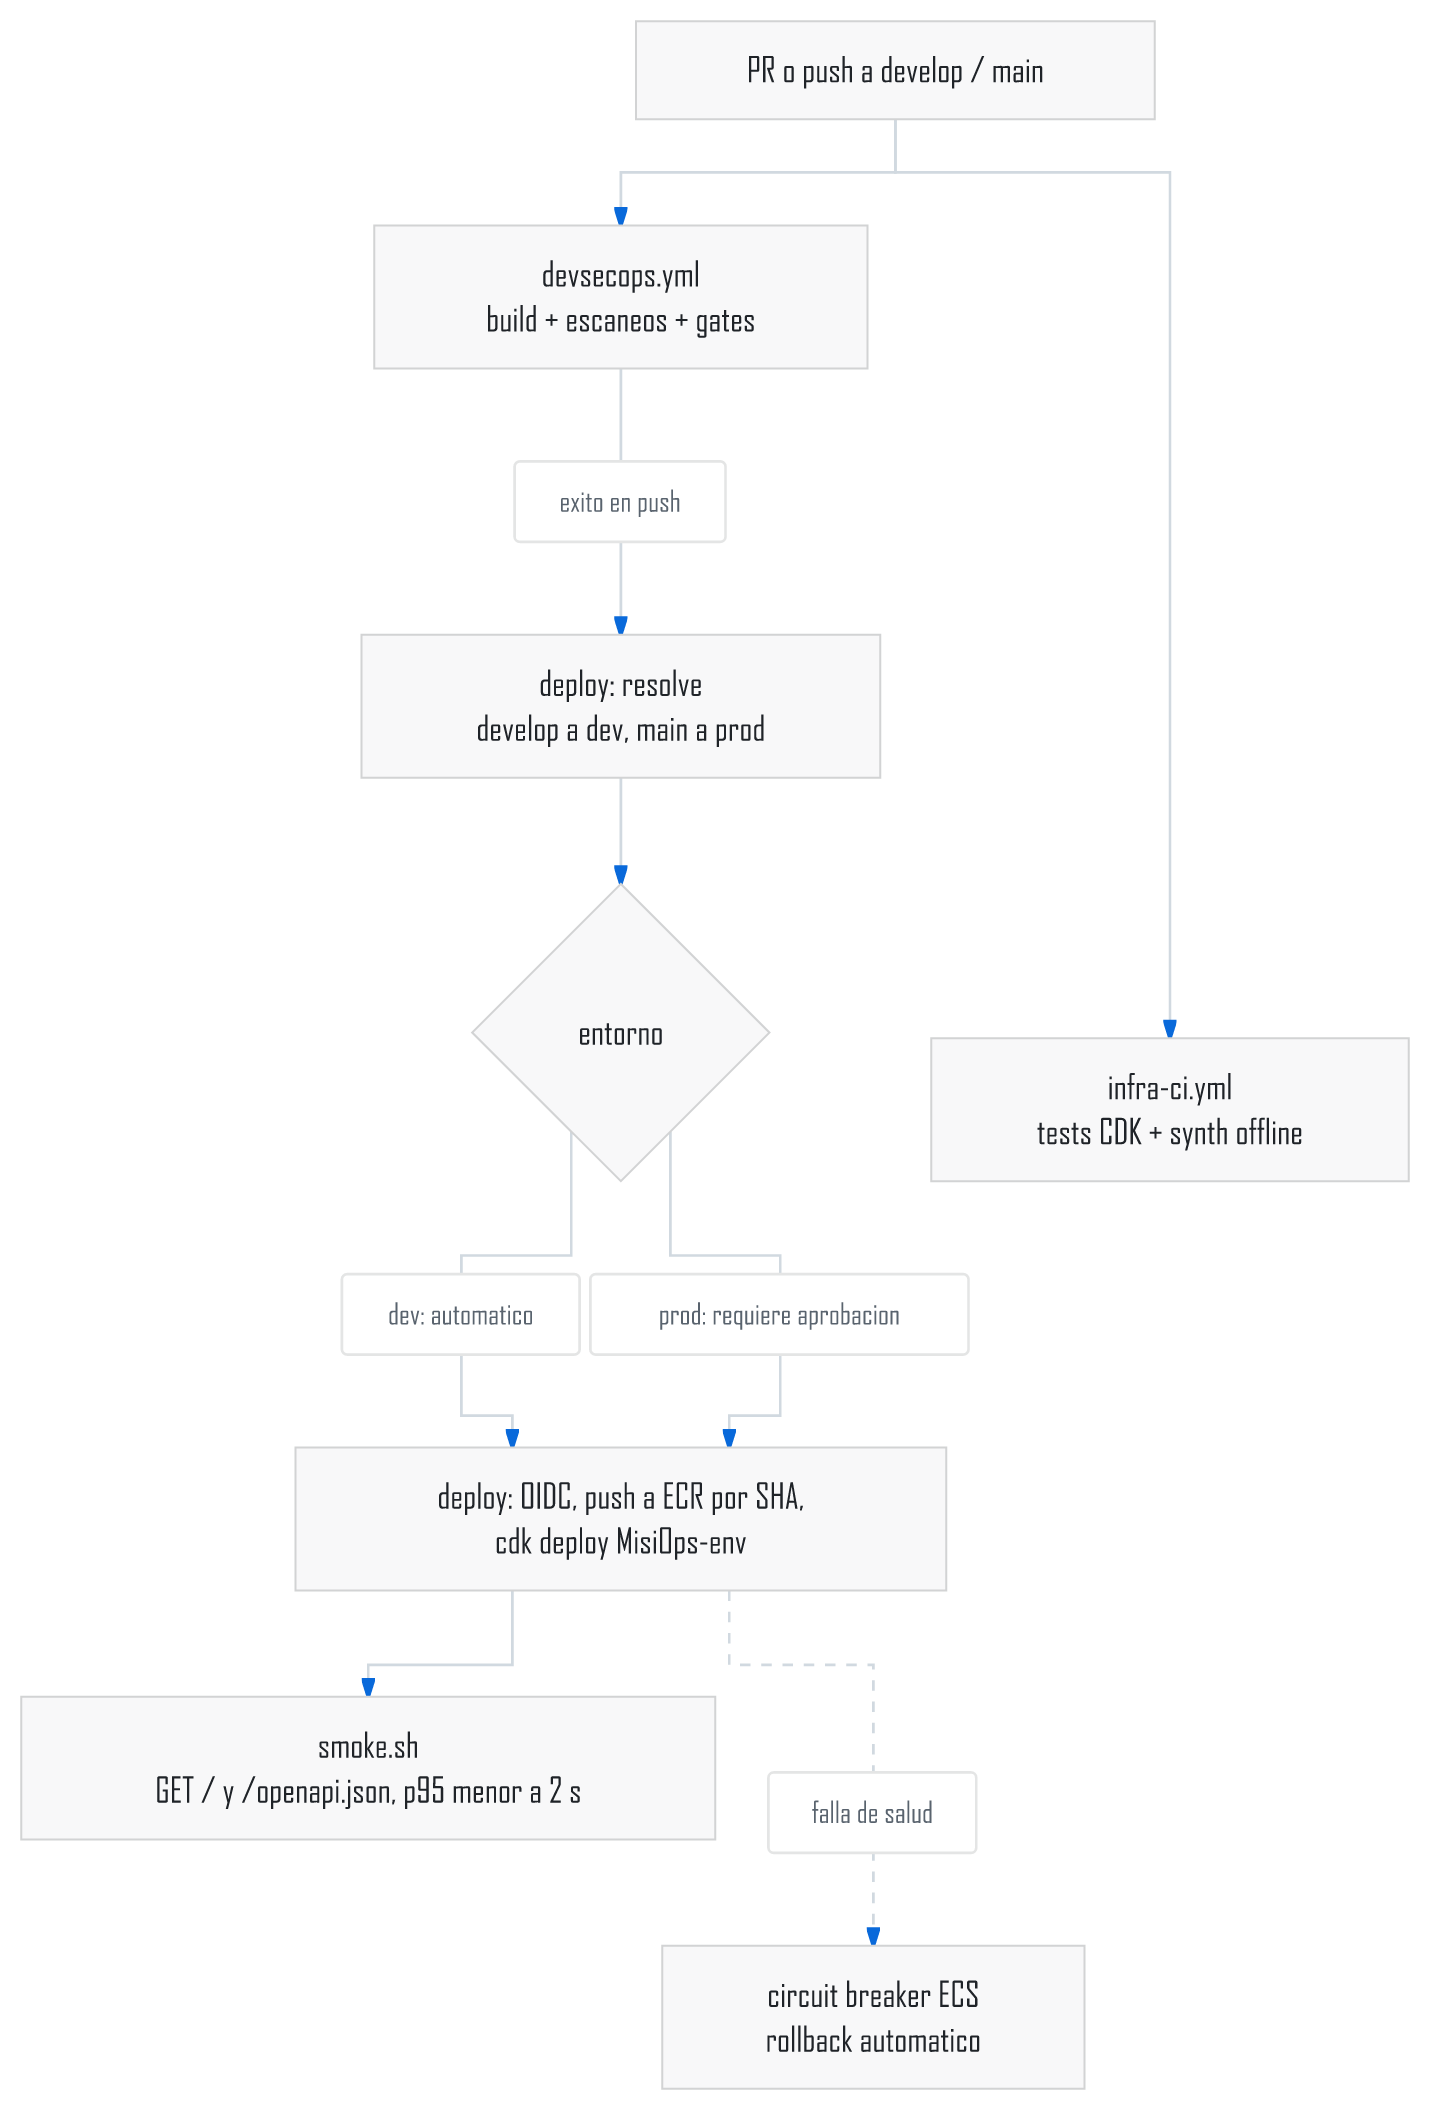
\includegraphics[width=0.55\textwidth]{figures/iac/iac-pipeline.png}
    \caption{Flujo de CI/CD de la infraestructura y del despliegue}
    \label{fig:iac-pipeline}
\end{figure}

\begin{enumerate}
    \item \textbf{\texttt{infra-ci.yml}} corre en cada PR o push a \texttt{develop} que toque \texttt{infra/}. Ejecuta los tests del CDK y un \textit{synth} sin credenciales de \texttt{dev} y \texttt{prod}, y comprueba que la plantilla no contenga ningún \texttt{SecretString}.
    \item \textbf{\texttt{devsecops.yml}} construye una sola vez las imágenes \texttt{linux/arm64}, las escanea y las guarda como artefacto (sección anterior).
    \item \textbf{\texttt{deploy.yml}} (Anexo~\ref{anx:deploy}) se dispara con \texttt{workflow\_run} cuando \texttt{devsecops} termina. Su job \texttt{resolve} solo continúa si la corrida fue un \textbf{push exitoso} y asigna \texttt{develop} $\rightarrow$ \texttt{dev} y \texttt{main} $\rightarrow$ \texttt{prod}. Los PR y las ejecuciones manuales nunca despliegan.
    \item El job \texttt{deploy} corre dentro del GitHub Environment correspondiente: \texttt{dev} es automático y \texttt{prod} espera la aprobación de un revisor. Después:
          \begin{itemize}
              \item asume el rol por OIDC;
              \item descarga el artefacto de imágenes de esa corrida, sin volver a construirlas;
              \item las sube a ECR con el SHA del commit;
              \item ejecuta \texttt{cdk deploy MisiOps-\textless env\textgreater};
              \item corre \texttt{infra/scripts/smoke.sh} contra la URL pública.
          \end{itemize}
    \item El resumen de la corrida registra entorno, commit, digest de ambas imágenes, URL pública, resultado del smoke test y duración. Los despliegues al mismo entorno se encolan (\texttt{concurrency: deploy-\textless env\textgreater}).
\end{enumerate}

\textbf{Rollback.} Si la nueva tarea no pasa el \textit{health check} del balanceador, el \textit{circuit breaker} de ECS vuelve a la definición de tarea anterior, CloudFormation deja el stack en \texttt{UPDATE\_ROLLBACK\_COMPLETE} y la corrida de \texttt{deploy} queda en rojo. Los usuarios siguen atendidos por la versión previa. Para un rollback manual se vuelve a ejecutar \texttt{devsecops} sobre el commit bueno, y eso redespliega esa versión por el mismo camino.

\subsection{Implementación en AWS CloudFormation}

\begin{itemize}
    \item \texttt{infra/bin/misiops.ts} crea la aplicación CDK: el stack \texttt{MisiOps-Foundation} y un \texttt{EnvironmentStack} según el contexto \texttt{-c env=dev|prod}.
    \item \texttt{infra/lib/environment-stack.ts} (unas 230 líneas) declara todos los recursos de un entorno. \texttt{infra/lib/config.ts} concentra las únicas diferencias entre \texttt{dev} y \texttt{prod}: la etiqueta ``dev'' visible en la interfaz, la política de borrado de la base de datos y la protección contra borrado.
    \item \texttt{cdk synth} produce las plantillas CloudFormation en \texttt{cdk.out/}; \texttt{cdk deploy} las envía a CloudFormation, que crea o actualiza los recursos y revierte si algo falla.
    \item \textbf{Pruebas}: 24 tests con \texttt{node:test} y \texttt{aws-cdk-lib/assertions} (20 del stack de entorno y 4 del stack Foundation). Verifican, entre otras cosas, la base de datos sin acceso público y cifrada, los secretos inyectados desde Secrets Manager, los tags inmutables en ECR, la condición de confianza OIDC y el \textit{circuit breaker} con rollback. A eso se suma un test en Bash del smoke script con un \texttt{curl} simulado.
\end{itemize}

Para que una misma imagen sirva en ambos entornos se hicieron dos cambios pequeños en la aplicación. El frontend llama a la API por rutas relativas del mismo dominio: el argumento de build \texttt{NEXT\_PUBLIC\_API\_BASE\_URL} vale vacío por defecto. Además muestra un banner y el sufijo ``· dev'' en el título solo cuando el contenedor tiene \texttt{APP\_ENV=dev}.

\subsection{Evidencias}

\textbf{Primer despliegue de \texttt{dev}} (manual, 2026-11-08). El primer intento de \texttt{cdk deploy MisiOps-dev} se revirtió automáticamente a los 14 minutos: el backend arrancó mientras Aurora seguía aprovisionándose y el \textit{circuit breaker} actuó sin dejar recursos huérfanos. Se corrigió haciendo que el servicio dependa de la base de datos. El segundo intento terminó en 9 minutos y el smoke test pasó, con p95 de 0.67 s en \texttt{GET /} y 0.62 s en \texttt{GET /openapi.json} sobre 20 peticiones. También se verificó de punta a punta el registro, el login, la creación de una transacción y su lectura en el resumen, a través de CloudFront y con los datos persistidos en Aurora.

\textbf{Despliegue automático de \texttt{prod}} (corrida \href{https://github.com/jeffreymonjacastro/MisiOps/actions/runs/43147540236}{43147540236}, 2026-11-12):
\begin{itemize}
    \item Se disparó tras la corrida verde de \texttt{devsecops} sobre \texttt{main} (merge del PR \#179, commit \texttt{8b85bc6}) y esperó la aprobación del revisor del entorno \texttt{prod}.
    \item \texttt{cdk deploy MisiOps-prod} creó el stack completo (52 recursos). El job tardó 10 min 31 s.
    \item URL pública: \url{https://dnowsrpw9uokx.cloudfront.net}.
    \item Smoke test: p95 de 0.175 s en \texttt{GET /} y de 0.098 s en \texttt{GET /openapi.json}.
    \item Digests publicados en ECR: backend \texttt{sha256:b3ed679f\ldots}, frontend \texttt{sha256:3cc14352\ldots}.
\end{itemize}

\begin{figure}[H]
    \centering
    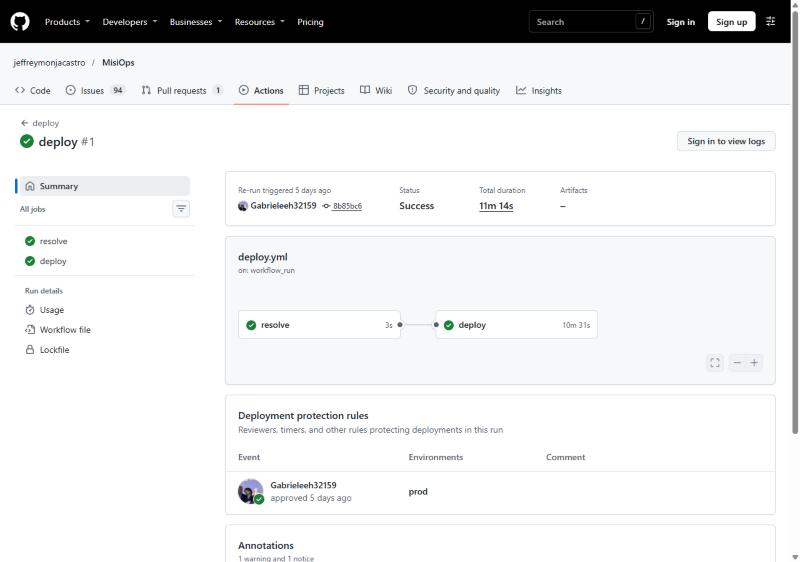
\includegraphics[width=0.9\textwidth]{figures/iac/deploy-run-prod.jpg}
    \caption{Corrida del workflow \texttt{deploy} hacia \texttt{prod}, con la aprobación registrada en las reglas de protección del entorno}
    \label{fig:deploy-prod}
\end{figure}

\begin{figure}[H]
    \centering
    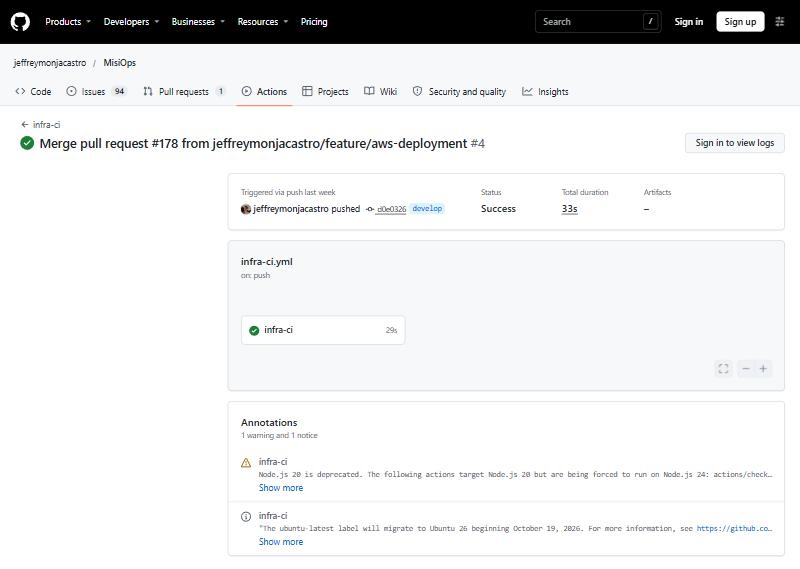
\includegraphics[width=0.9\textwidth]{figures/iac/infra-ci-run.jpg}
    \caption{Corrida de \texttt{infra-ci} (tests del CDK y \textit{synth}) tras el merge del PR \#178 a \texttt{develop}}
    \label{fig:infra-ci}
\end{figure}

\begin{figure}[H]
    \centering
    \begin{minipage}{0.49\textwidth}
        \centering
        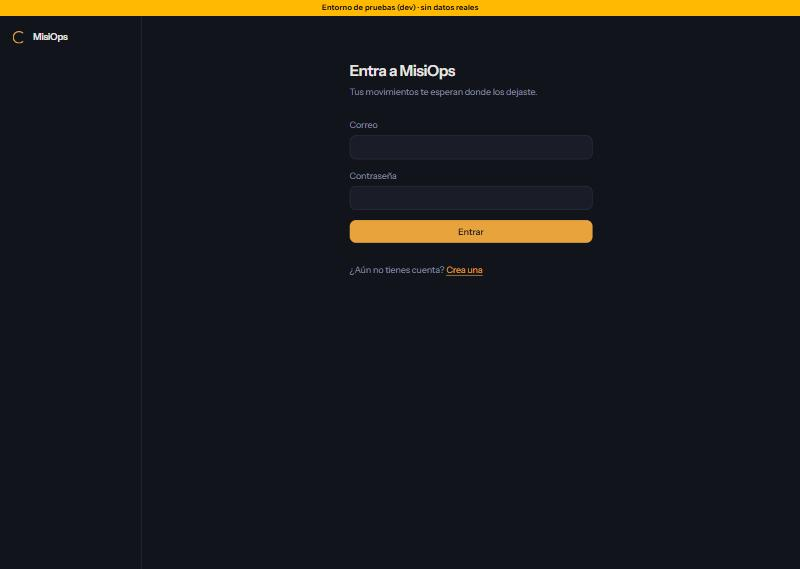
\includegraphics[width=\linewidth]{figures/iac/app-dev.jpg}
        \small (a) \texttt{dev}: \url{https://d2n2ap8z1x33no.cloudfront.net}
    \end{minipage}
    \hfill
    \begin{minipage}{0.49\textwidth}
        \centering
        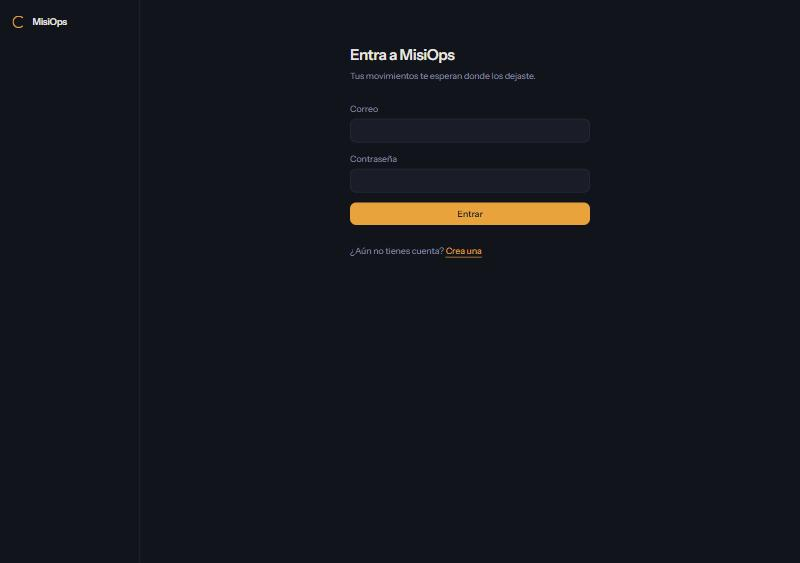
\includegraphics[width=\linewidth]{figures/iac/app-prod.jpg}
        \small (b) \texttt{prod}: \url{https://dnowsrpw9uokx.cloudfront.net}
    \end{minipage}
    \caption{MisiOps desplegado en AWS: \texttt{dev} muestra el banner de entorno de pruebas y \texttt{prod} no}
    \label{fig:apps}
\end{figure}

La guía de operación completa (preparación de la cuenta, aprobación de \texttt{prod}, rollback, logs, costos y destrucción del entorno) está en \texttt{docs/deployment/README.md}.
